\chapter{Onderzoek}

Zoals in de opdrachtomschrijving op pagina \pageref{opdracht} te zien is, was het noodzakelijk om een aantal onderzoeken uit te voeren, aan de hand van welke besluiten genomen konden worden. In dit hoofdstuk komen al deze onderzoeken aan bod, met hun uitvoering en conclusies.

\section{CAN Hardware}

Een van de eerste onderzoeken was een analyse van de huidig beschikbare CAN hardware, die de verbinding tussen de CAN bus en de PC verzorgen.

Een eis was wel, mocht er ooit besloten worden andere hardware aan te schaffen, het mogelijk moest zijn hier makkelijk een driver voor te maken. Dit is opgelost door een generieke architectuur te ontwerpen, die later toegelicht zal worden.

Op internet heb ik de specificaties opgezocht van een aantal leveranciers van CAN hardware en hiervan een duidelijk overzicht gemaakt. Ook de \index{API}API werdt hierbij onder de loep genomen, om er zeker van te zijn dat software daadwerkelijk aansloot bij de hardware.

De uiteindelijke conclusie hier was, dat de huidige Softing CANusb dongel prima geschikt was voor de Delem toepassingen. Er waren veel luxere en minder luxe te krijgen, maar omdat er hier al enkelen van in het bezit van Delem zijn, is er besloten deze te gebruiken.

\section{Definitie}
\label{definitie}

Zoals in de opdrachtomschrijving te vinden is, was een verdere eis het omschrijven van de HSB commando's in een eenvoudig formaat. Dit formaat moest makkelijk uitbreidbaar zijn, zonder in de knoop te raken met bestaande definities.

Om dit te realiseren werd door een ontwikkelaar \index{XML}XML voorgesteld. Om te kijken of die geschikt was, is er eerst gekeken wat voor zaken er gespecifeerd dienden te worden om alle commando's eenduidig te kunnen identificeren.

Nadat dit bekend werd, is er een voorbeeld XML bestand gemaakt met wat commando's erin en via \index{XSLT}XSLT omgezet naar C structuren, die door een preprocessor module toegepast word op de inkomende gegevensstroom.

De versie die dit ondersteunde is omgedoopt tot prototype en is uitvoerig besproken met de bedrijfsbegeleider. Deze was dusdanig enthousiast dat er besloten is op deze manier door te gaan.

Hierna is er gekeken om deze definities ook naar HTML te converteren, als documentatie. Toen later bleek dat je met een HTML bestand en een HHC\footnote{Inhoudsopgave bestand voor een CHM file} file een CHM file kan maken is ervoor gekozen om dit als help formaat binnen de applicatie te gebruiken, zodat commando's makkelijker op te zoeken zijn.

Het was uiteindelijk ook de bedoeling om het bestaande document met commando's te kunnen genereren vanuit de definitie. Dit overzicht zal aan het bestaande document toegevoegd worden, als een appendix. De definities worden weer door XSLT geprocessed, maar dan naar \LaTeX\mbox{-}formaat. Dat laatste wordt door \LaTeX\mbox{-}uiteindelijk geprocessed naar een PDF bestand, dat netjes uit te printen is.

Later is er ook gekeken naar de mogelijkheid om deze definities rechtstreeks uit de XML file zelf te lezen. Na een korte vergelijking tussen MSXML en libxml2 is er gekozen voor de laatste, aangezien MSXML zeer omslachtig in het gebruik is. Verder is de documentatie van libxml2 veel beter en kon er meteen mee aan de slag worden gegaan. Het resultaat is dat je definities voortaan kunt aanpassen zonder het programma opnieuw te moeten compileren.

\newpage
\subsection{Overzicht}

Uiteindelijk ziet het overzicht van het XML-transformatie proces er als volgt uit:

\begin{figure}[h]
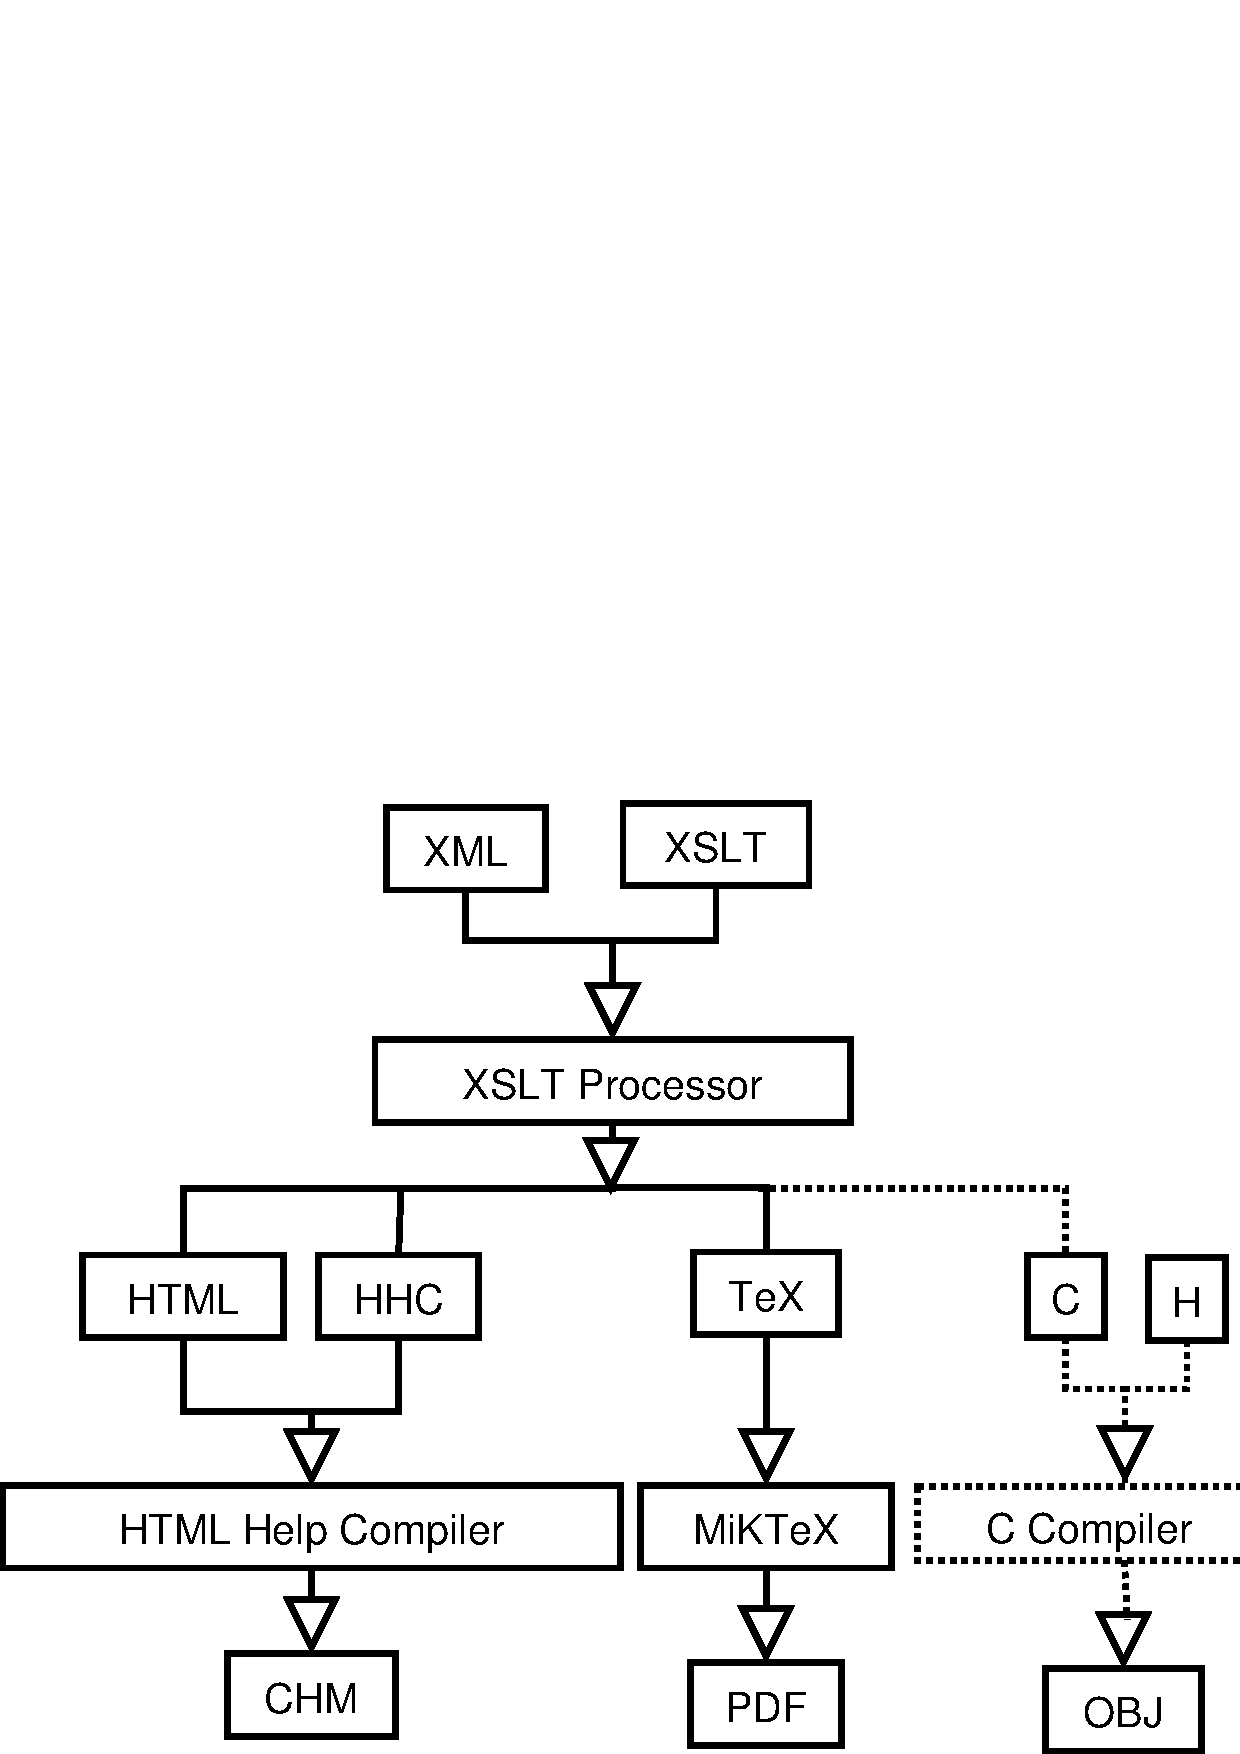
\includegraphics[width=\textwidth]{xml.pdf}
\end{figure}

In dit overzicht is het C-gedeelte met stippellijnen aangeduid, omdat dit stuk later kwam te vervallen.

\section{Uitbreidbaarheid}

Aan het einde van het project bleek dat er een extreem grote behoefte was tot het eenvoudig ontwikkelen van plugins, die ervoor zorgen dat de huidige functionaliteit eenvoudig uit te breiden is. Er werden twee mogelijkheden bekeken: scripts en DLL bestanden.

Het voordeel van scripts was dat ze erg makkelijk te maken en onderhouden zijn. Helaas was de verwachting dat het realtime gedrag niet meer gegarandeerd kan worden als er voor een dusdanige oplossing gekozen zou worden. Daarom is deze oplossing verder dus niet verder onderzocht.

DLL bestanden leken ideaal: het is gewoon C++ code, je kunt bestaande code recycelen. Nadat er dan ook een goede API ontworpen was, die later flink uitgebreid is, is dit dan ook gepresenteerd aan de ontwikkelaars. Deze API werkt prima en er zijn geen verschillen bemerkbaar in snelheid.
